\documentclass[12pt]{article}

\usepackage{graphicx}
\usepackage{paralist}
\usepackage{amsfonts}
\usepackage{hyperref}
\usepackage{listings}
\usepackage{subfig}
\usepackage{float}

\oddsidemargin 0mm
\evensidemargin 0mm
\textwidth 160mm
\textheight 200mm
\renewcommand\baselinestretch{1.0}

\pagestyle {plain}
\pagenumbering{arabic}
\newcounter{stepnum}

\title{Course Project}
% \author{Hyosik Moon}
\author{
  Moon, Hyosik
  }

\begin {document}

\maketitle

\section{Required}

\begin{itemize}
\item \textbf{Main objective of the analysis} \\
We will optimize the `CartPole-v0' problem with three different models such as `RandomForestRegressor, AdaBoostRegressor, ExtraTreesRegressor'. The goal of the problem is to prevent a pole attached to a cart from falling over by increasing and reducing the cart's velocity. Whenever it successes to mainatain the pole, it gets a socre as a reward. We win the game, if we maintain the pole for 200 times.

\item \textbf{Brief description of the data set} \\
Because this is reinforcement problem we need to produce our own data set. In order to get the data set, I implemented the game 1000 times. We can check the data in the figure \ref{data}.

\begin{figure}[H]
    \centering
    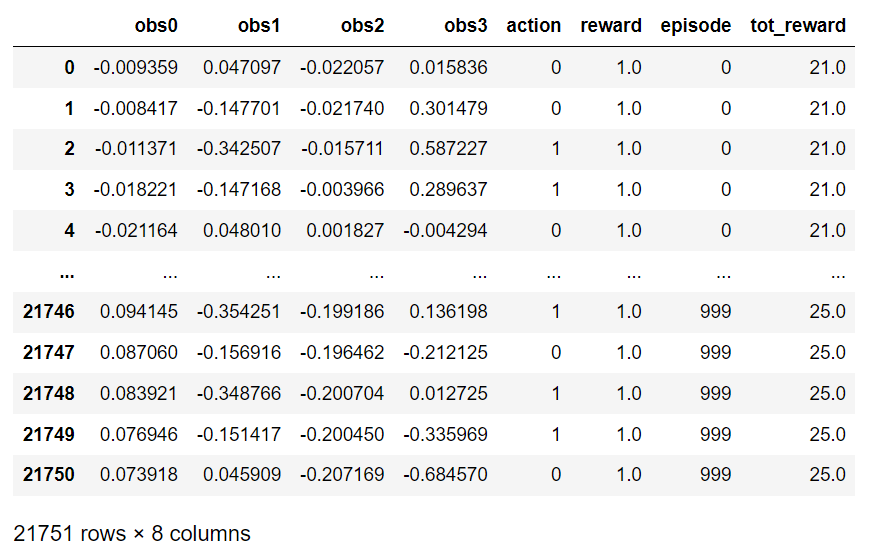
\includegraphics[width=0.9\textwidth]{figures/data.png}
    \caption{Data set information}\label{data}
\end{figure}

\item \textbf{Brief summary of data exploration}
In order to train a model, we need the pole's positions, actions, and reward. So we just manipulate the data a little bit as `x = positions, action', and 'y = reward'.
    
    % \begin{figure}[H]
    %   \centering
    %   \subfloat[Correlation]{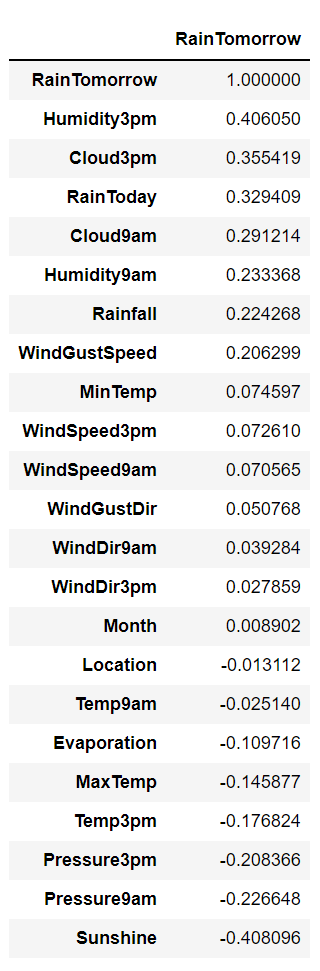
\includegraphics[width=0.3\textwidth]{figures/corr.png}\label{corr}}
    %   \hfill
    %   \subfloat[Correlation bar plot]{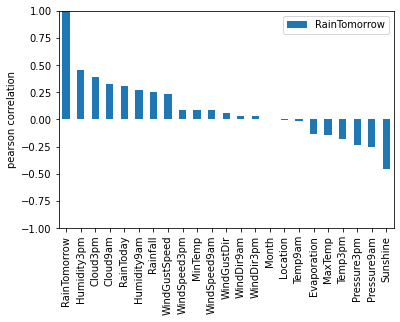
\includegraphics[width=0.65\textwidth]{figures/corr2.png}\label{corr2}}
    % \end{figure}

\item \textbf{Summary of training at least three linear regression models} I implemented three different prediction models which are Linear Regression, Support Vector Machine, and Random Forest. And in order to regularize the models I also used cross validation.
    \begin{enumerate}
      \item LinearRegressionCV. The weighted f1-score and accuracy of the model were 0.846, 0.855 respectively. I trained the model by using stratified shuffle split because the target was skewed to 0 (No rain) (Figure \ref{lr_l1}, \ref{lr_l1_cm}).
    \end{enumerate}

    \begin{figure}[H]
      \centering
      \subfloat[Evaluation metrics for LRCV]{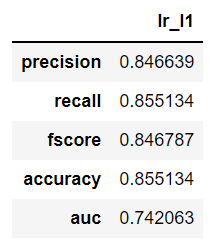
\includegraphics[width=0.4\textwidth]{figures/lr_l1.png}\label{lr_l1}}
      \hfill
      \subfloat[Confusion metrics]{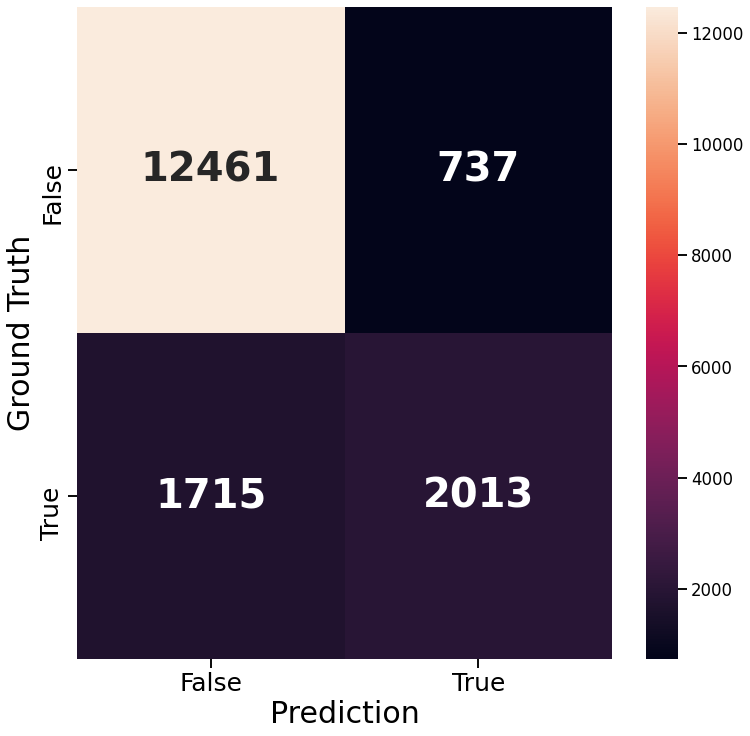
\includegraphics[width=0.5\textwidth]{figures/lr_l1_cm.png}\label{lr_l1_cm}}
    \end{figure}

    \item Support Vector Machine. The weighted f1-score and accuracy of the model were 0.846, 0.858 respectively. As a kernel function, I used rbf (Radial Basis Function) (Figure \ref{svmg}, \ref{svmg_cm}).

    \begin{figure}[H]
      \centering
      \subfloat[Evaluation metrics for SVM\_Gaussian]{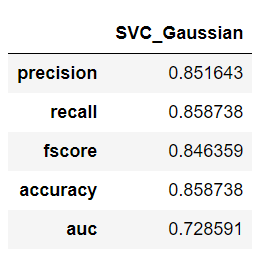
\includegraphics[width=0.4\textwidth]{figures/svmg.png}\label{svmg}}
      \hfill
      \subfloat[Confusion metrics]{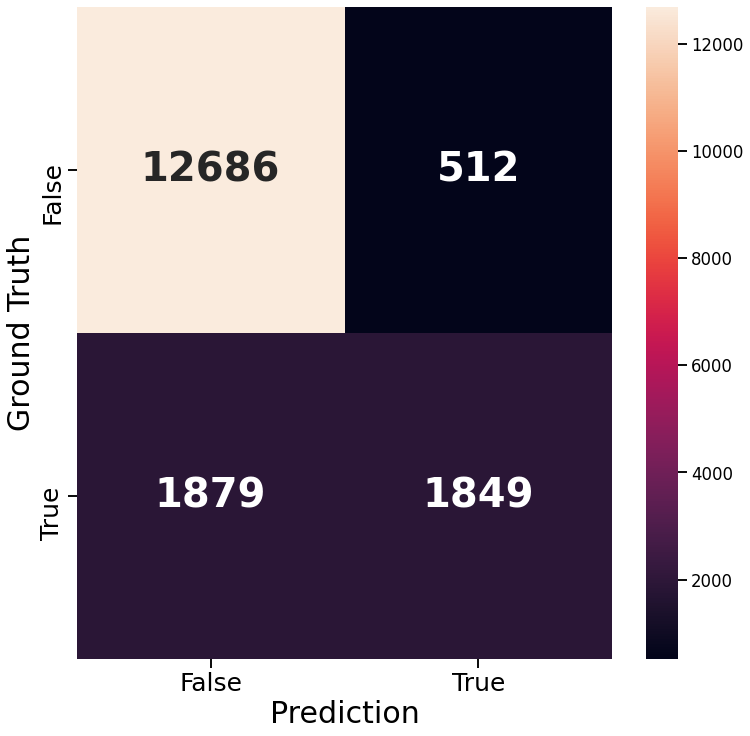
\includegraphics[width=0.5\textwidth]{figures/svmg_cm.png}\label{svmg_cm}}
    \end{figure}

    \item Random Forest. The weighted f1-score and accuracy of the model were 0.854, 0.864 respectively, and to find the best number of trees, out-of-error scores were used. And then the model use the 400 trees to predic the RainTomorrow (Figure \ref{rf}, \ref{rf_cm}, \ref{rfe}).

    \begin{figure}[H]
      \centering
      \subfloat[Evaluation metrics for Random Forest]{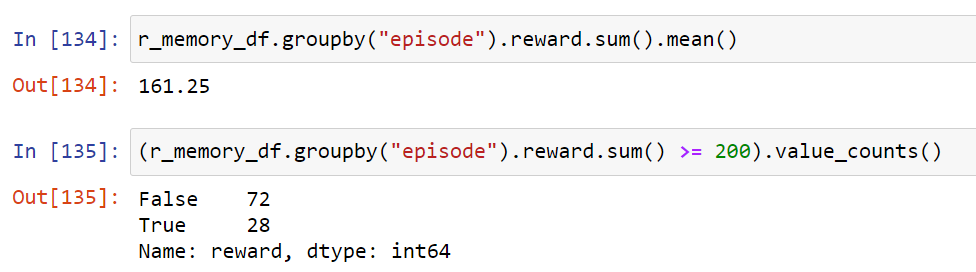
\includegraphics[width=0.4\textwidth]{figures/rf.png}\label{rf}}
      \hfill
      \subfloat[Confusion metrics]{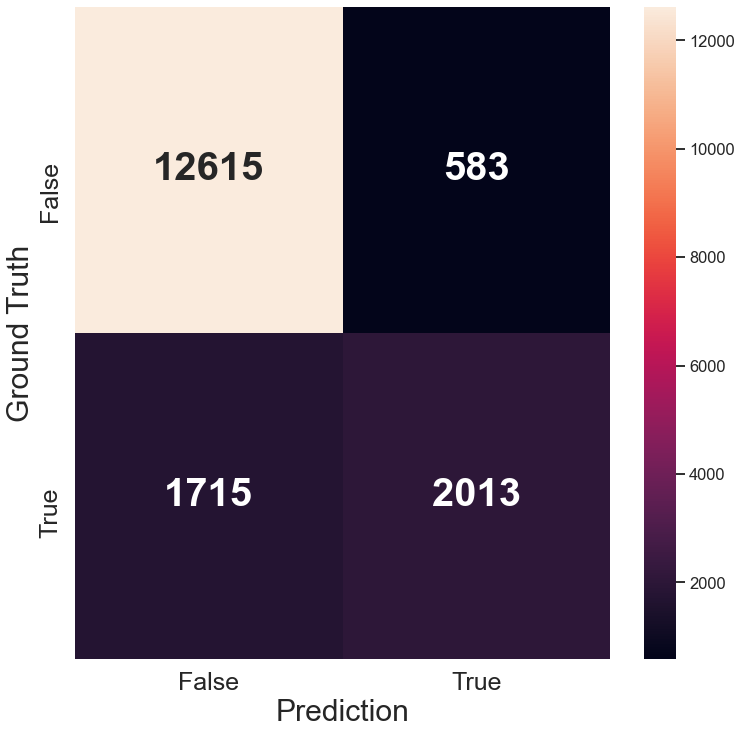
\includegraphics[width=0.5\textwidth]{figures/rf_cm.png}\label{rf_cm}}
    \end{figure}

    \begin{figure}[H]
      \centering
      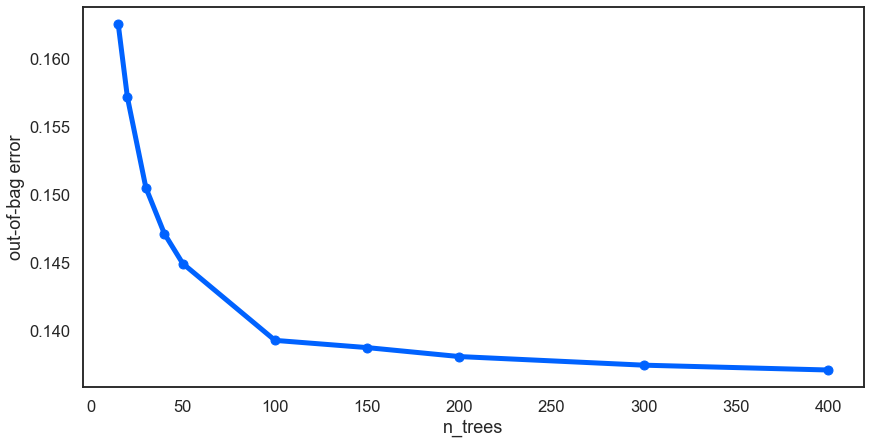
\includegraphics[width=0.8\textwidth]{figures/rfe.png}
      \caption{Out of error scores}\label{rfe}
    \end{figure}

\item \textbf{Explanation of your final regressions model}
Overall, all models showed the similar f1-score and accuracy. The best one was Random Forest which has the fscore	0.854873 and accuracy	0.864233. The ROC, Precision\_Recall curve accuracies aren't quite ideal.
This is because the RainTomorrow is unbalanced. For example, `No (rain)' takes about 77\%, `Yes (rain)' takes about 23\%. As a result the model predict the RainTomorrow relatively close to `No (rain)' even though the ground truth is `Yes (rain)'. It leads to relatively low ROC and Precision\_Recall curve accuracies (Figure \ref{roc_pr}).

\begin{figure}[H]
  \centering
  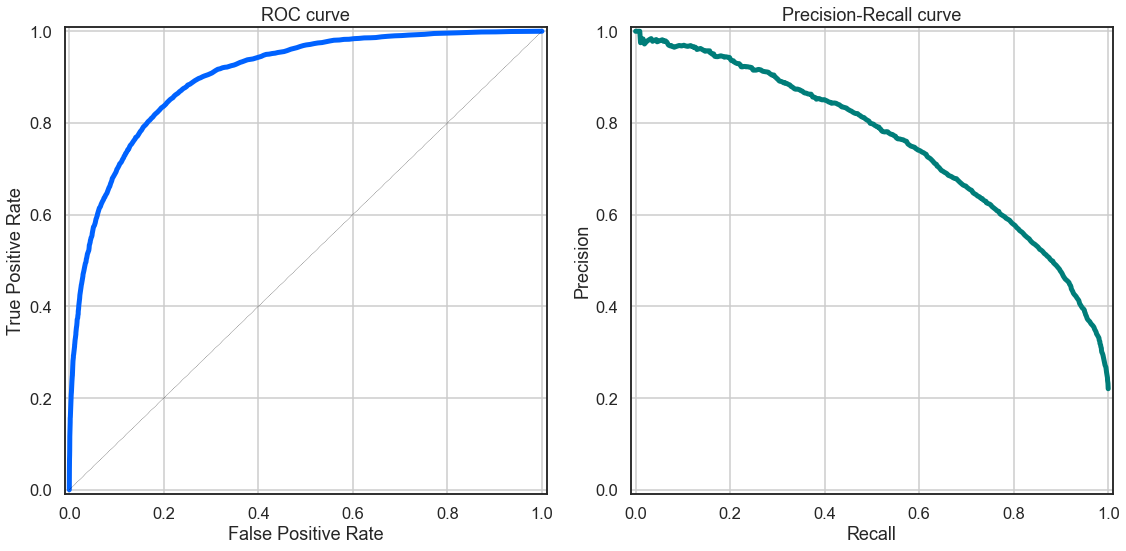
\includegraphics[width=0.8\textwidth]{figures/roc_pr.png}
  \caption{ROC, Pricision-Recall curves}\label{roc_pr}
\end{figure}

\item \textbf{Summary Key Findings and Insights}
The fact that the accuracies among the models are similir means that the reliability of the models is also high. And the three most important features to predic the RainTomorrow are `Hymidity3pm, Sunshine, and Pressure3pm'. These features are similir to the features that had high correlation values (Figrue \ref{imp}). As a result, we can conclude that `Hymidity3pm, Sunshine, and Pressure3pm' are the most important factores to predict the tomorrow's rain and with more features we can predict the tomorrows rain with 86\% accuracy.

\begin{figure}[H]
  \centering
  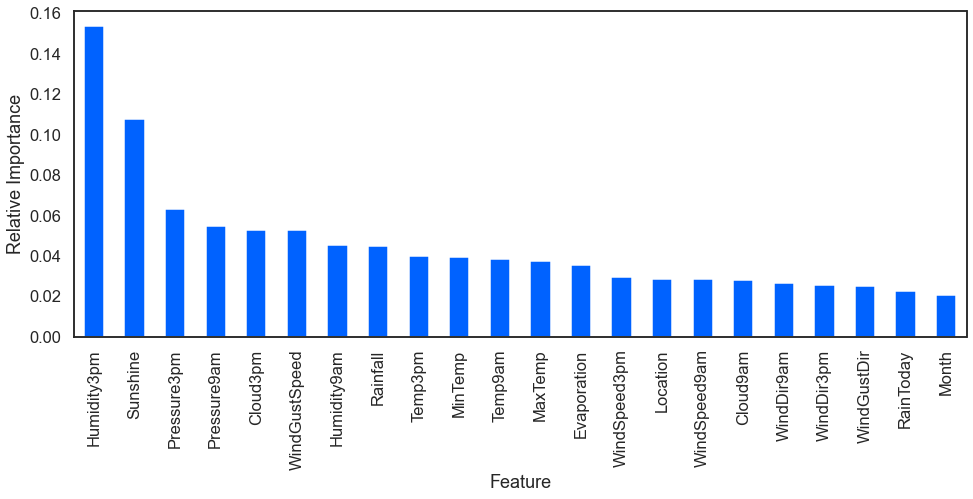
\includegraphics[width=0.8\textwidth]{figures/feature_imp.png}
  \caption{Feature importance}\label{imp}
\end{figure}

\item \textbf{Suggestions for next steps}
If the data were balanced, then we might predict more accuracte data. So, manipulating the unbalanced data will be a good-next step to imporve the model.

\end{itemize}

\end {document}